% ============================================================
% CAPITULO 20: DIFERENCIACION PARCIAL, PLANO TANGENTE Y DIFERENCIABILIDAD
% ============================================================

\chapter{Diferenciación parcial, plano tangente y diferenciabilidad}

El capítulo anterior estableció los conceptos de límite y continuidad para
funciones de varias variables. El paso natural siguiente es extender la
noción de \textbf{derivada}: para una función $f(x,y)$, ¿cómo varía $f$
cuando $x$ cambia y $y$ permanece fijo? Esta pregunta conduce a la
\textbf{derivada parcial}. Con ella se construye el \textbf{plano tangente}
—la aproximación lineal de una superficie en un punto— y se formula la
\textbf{diferenciabilidad}, que es más exigente que la mera existencia de
las derivadas parciales: una función puede tener todas sus derivadas
parciales y aun así no ser diferenciable.

% ============================================================
% SECCIÓN 1.4: DERIVADAS PARCIALES DE PRIMER ORDEN Y ORDEN SUPERIOR
% ============================================================

\section{Derivadas parciales}

La derivada de una función de una variable mide la tasa de cambio
instantánea cuando la variable independiente varía. Para una función
de dos variables, la pregunta natural es: ¿cómo cambia $f$ cuando
solo una de las variables varía y la otra permanece fija? Esta
pregunta conduce al concepto de derivada parcial: la derivada con
respecto a una variable, manteniendo las demás constantes.

\begin{definition}[Derivadas parciales primeras]
Sea $f$ una función de dos variables. Las \textbf{derivadas parciales
de primer orden} de $f$ en $(x,y)$ se definen como:
\[
f_x(x,y) = \frac{\partial f}{\partial x}
= \lim_{h\to 0} \frac{f(x+h,y)-f(x,y)}{h},
\]
\[
f_y(x,y) = \frac{\partial f}{\partial y}
= \lim_{h\to 0} \frac{f(x,y+h)-f(x,y)}{h},
\]
siempre que los límites existan.
\end{definition}

La notación $\frac{\partial f}{\partial x}$ (introducida por
Jacobi) distingue la derivada parcial de la derivada ordinaria
$\frac{df}{dx}$. La letra $\partial$ se lee ``derivada parcial de''.

\begin{rem}
Operativamente, para calcular $f_x$ se deriva $f$ como si $y$ fuera
una constante; para calcular $f_y$, se deriva como si $x$ fuera
constante. Todas las reglas de derivación de una variable (producto,
cociente, cadena, etc.) se aplican normalmente, tratando a la otra
variable como constante.
\end{rem}

% ------------------------------------------------------------
% INTERPRETACIÓN GEOMÉTRICA
% ------------------------------------------------------------

Las derivadas parciales tienen una interpretación geométrica clara.
Dada la superficie $z=f(x,y)$, consideremos el plano $y=y_0$, que
corta a la superficie en una curva $C$. La derivada parcial
$f_x(x_0,y_0)$ es la pendiente de la recta tangente a esa curva en
el punto $(x_0,y_0,f(x_0,y_0))$. Análogamente, $f_y(x_0,y_0)$ es la
pendiente de la recta tangente a la curva obtenida al cortar con el
plano $x=x_0$.

\begin{figure}[H]
\centering
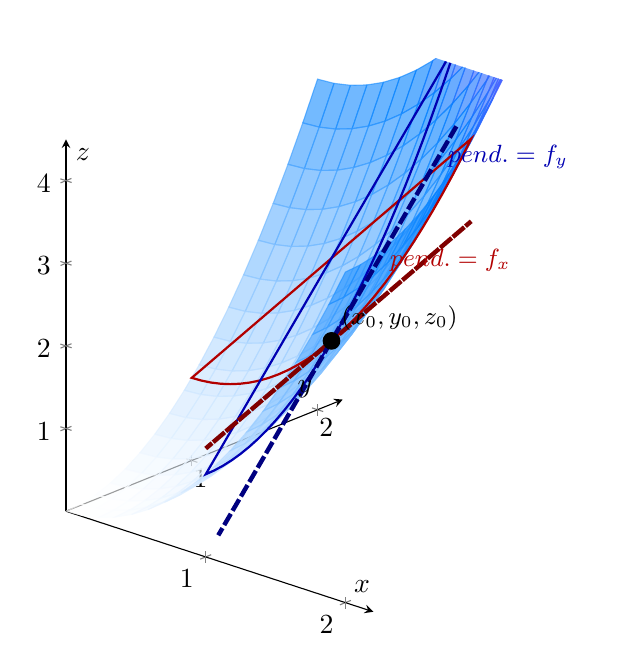
\begin{tikzpicture}
\begin{axis}[
    view={42}{22},
    xlabel={$x$}, ylabel={$y$}, zlabel={$z$},
    axis lines=center,
    tick style={thin},
    zmin=0, zmax=4.5,
    xmin=0, xmax=2.2,
    ymin=0, ymax=2.2,
    xtick={1,2}, ytick={1,2}, ztick={1,2,3,4},
    width=9cm, height=9cm,
]
    % Superficie z = x^2 + y^2
    \addplot3[
        surf, shader=flat corner,
        samples=18, domain=0:2, y domain=0:2,
        opacity=0.62, colormap/cool,
    ] {x^2 + y^2};
    % Curva de corte con y=y0=1 (roja, sobre la superficie)
    \addplot3[thick, red!70!black, variable=t, domain=0:2, samples=30]
        ({t}, {1}, {t*t + 1});
    % Curva de corte con x=x0=1 (azul, sobre la superficie)
    \addplot3[thick, blue!70!black, variable=t, domain=0:2, samples=30]
        ({1}, {t}, {1 + t*t});
    % Recta tangente en x (pendiente f_x=2): z = 2x, y=1 fijo
    \addplot3[ultra thick, red!50!black, dashed, variable=t, domain=0.1:2.0, samples=2]
        ({t}, {1}, {2*t});
    % Recta tangente en y (pendiente f_y=2): z = 2y, x=1 fijo
    \addplot3[ultra thick, blue!50!black, dashed, variable=t, domain=0.1:2.0, samples=2]
        ({1}, {t}, {2*t});
    % Punto de tangencia (1,1,2)
    \addplot3[only marks, mark=*, mark size=3pt, black]
        coordinates {(1,1,2)};
    \node[anchor=south west, black] at (axis cs:1,1,2)
        {\small $(x_0,y_0,z_0)$};
    % Etiquetas rectas tangentes
    \node[anchor=north, red!70!black] at (axis cs:1.85,1,3.7)
        {\small $\text{pend.}=f_x$};
    \node[anchor=west, blue!70!black] at (axis cs:1,1.85,3.7)
        {\small $\text{pend.}=f_y$};
\end{axis}
\end{tikzpicture}
\caption{Interpretación geométrica de las derivadas parciales: la curva roja (corte $y=y_0$) tiene recta tangente (roja punteada) con pendiente $f_x(x_0,y_0)$; la curva azul (corte $x=x_0$) tiene recta tangente (azul punteada) con pendiente $f_y(x_0,y_0)$.}
\label{fig:dp_interpretacion_geometrica}
\end{figure}

\begin{example}[Derivadas parciales por definición]
Calcular las primeras derivadas parciales de $f(x,y)=x^2 y^3$ usando
la definición.
\begin{myproof}
\textbf{Paso 1. Derivada parcial con respecto a $x$.}
\begin{align*}
f_x(x,y) = \lim_{h\to 0} \frac{(x+h)^2 y^3 - x^2 y^3}{h}\\
&= \lim_{h\to 0} \frac{(x^2+2xh+h^2)y^3 - x^2 y^3}{h}
= \lim_{h\to 0} \frac{2xhy^3 + h^2 y^3}{h}\\
&= \lim_{h\to 0} (2xy^3 + h y^3)
= 2xy^3.
\end{align*}



\textbf{Paso 2. Derivada parcial con respecto a $y$.}
\[
f_y(x,y) = \lim_{h\to 0} \frac{x^2(y+h)^3 - x^2 y^3}{h}
= \lim_{h\to 0} \frac{x^2(y^3+3y^2h+3yh^2+h^3) - x^2y^3}{h}
\]
\[
= \lim_{h\to 0} \frac{x^2(3y^2h+3yh^2+h^3)}{h}
= \lim_{h\to 0} x^2(3y^2+3yh+h^2)
= 3x^2y^2.
\]

\textbf{Paso 3. Verificación con reglas directas.}
Tratando $y$ como constante: $\partial_x(x^2y^3)=2xy^3$ ✓. Tratando $x$ como constante: $\partial_y(x^2y^3)=3x^2y^2$ ✓.

\textbf{Paso 4. Resultado.}
\[
\boxed{f_x(x,y)=2xy^3,\qquad f_y(x,y)=3x^2y^2}
\]
\end{myproof}
\end{example}

\begin{rem}
En la práctica, rara vez se usan los límites para calcular derivadas
parciales; se aplican directamente las reglas de derivación
ordinarias tratando a la otra variable como constante.
\end{rem}

\begin{example}[Derivadas parciales por reglas operativas]
Calcular las primeras derivadas parciales de:
\begin{enumerate}[a)]
    \item $f(x,y)=x e^{x/y}$,
    \item $f(x,y)=\ln(x^2+y^2)$.
\end{enumerate}
\begin{myproof}
\textbf{Paso 1. Función (a) $f(x,y)=x e^{x/y}$ — regla del producto y de la cadena.}

$f_x$ ($y$ constante, regla del producto):
\[
f_x = 1\cdot e^{x/y} + x\cdot e^{x/y}\cdot \frac{1}{y}
= e^{x/y}\left(1+\frac{x}{y}\right).
\]

\textbf{Paso 2. Función (a): $f_y$ y resultado.}

$f_y$ ($x$ constante, cadena sobre $e^{x/y}$):
\[
f_y = x e^{x/y}\cdot \left(-\frac{x}{y^2}\right)
= -\frac{x^2}{y^2} e^{x/y}.
\]
\[
\boxed{f_x = e^{x/y}\!\left(1+\frac{x}{y}\right),\qquad
f_y = -\frac{x^2}{y^2}e^{x/y}}
\]

\textbf{Paso 3. Función (b) $f(x,y)=\ln(x^2+y^2)$ — logaritmo compuesto.}

$f_x$ ($y$ constante):
$f_x = \dfrac{2x}{x^2+y^2}$.
\quad
$f_y$ ($x$ constante):
$f_y = \dfrac{2y}{x^2+y^2}$.

\textbf{Paso 4. Resultado de (b).}
\[
\boxed{f_x = \frac{2x}{x^2+y^2},\qquad
f_y = \frac{2y}{x^2+y^2}}
\]
\end{myproof}
\end{example}

\begin{example}[Estimación de derivadas parciales a partir de una tabla]
La tabla registra la \emph{sensación térmica} $S$ (en $^\circ$C) en función de
la temperatura del aire $T$ (en $^\circ$C) y la velocidad del viento $v$ (en
km/h) medidas en una estación meteorológica:
\begin{center}
\begin{tabular}{c|cccc}
$S(T,v)$ & $v=10$ & $v=20$ & $v=30$ & $v=40$ \\ \hline
$T=-10$  & $-15$  & $-18$  & $-20$  & $-21$  \\
$T=-5$   & $-9$   & $-12$  & $-14$  & $-15$  \\
$T=0$    & $-3$   & $-5$   & $-7$   & $-8$   \\
$T=5$    & $3$    & $1$    & $-1$   & $-2$   \\
\end{tabular}
\end{center}
Estime $\partial S/\partial T$ y $\partial S/\partial v$ en el punto
$(T,v)=(-5,20)$ e interprete sus unidades y signos.
\begin{myproof}
\textbf{Paso 1. Las parciales como cociente incremental.}
Cada parcial es el límite de un cociente incremental; con datos tabulados lo
aproximamos por \emph{diferencias centradas} (promediando los dos lados) a
partir de los valores vecinos en la misma columna o fila.

\textbf{Paso 2. $\partial S/\partial T$ en $(-5,20)$ (columna $v=20$ fija).}
Con las filas vecinas $T=-10$ y $T=0$:
\[
  \frac{\partial S}{\partial T}\approx
  \frac{S(0,20)-S(-10,20)}{0-(-10)}
  =\frac{-5-(-18)}{10}=\frac{13}{10}=1.3.
\]

\textbf{Paso 3. $\partial S/\partial v$ en $(-5,20)$ (fila $T=-5$ fija).}
Con las columnas vecinas $v=10$ y $v=30$:
\[
  \frac{\partial S}{\partial v}\approx
  \frac{S(-5,30)-S(-5,10)}{30-10}
  =\frac{-14-(-9)}{20}=\frac{-5}{20}=-0.25.
\]

\textbf{Paso 4. Interpretación.}
\[
  \boxed{\ \frac{\partial S}{\partial T}\approx 1.3,\qquad
  \frac{\partial S}{\partial v}\approx -0.25\ \tfrac{^\circ\text{C}}{\text{km/h}}.\ }
\]
$\partial S/\partial T>0$: al subir la temperatura del aire aumenta la
sensación térmica (algo amplificada, $1.3\,^\circ$C por cada $^\circ$C).
$\partial S/\partial v<0$: más viento produce una sensación más fría, a razón
de unos $0.25\,^\circ$C por cada km/h adicional.
\end{myproof}
\end{example}

% ------------------------------------------------------------
% DERIVADAS PARCIALES DE ORDEN SUPERIOR
% ------------------------------------------------------------

\begin{definition}[Derivadas parciales de segundo orden]
Si $f$ tiene derivadas parciales primeras, podemos derivarlas de
nuevo para obtener las \textbf{derivadas parciales de segundo orden}:
\[
\begin{aligned}
f_{xx} &= \frac{\partial^2 f}{\partial x^2}
       = \frac{\partial}{\partial x}\left(\frac{\partial f}{\partial x}\right),\\
f_{xy} &= \frac{\partial^2 f}{\partial y\partial x}
       = \frac{\partial}{\partial y}\left(\frac{\partial f}{\partial x}\right),\\
f_{yx} &= \frac{\partial^2 f}{\partial x\partial y}
       = \frac{\partial}{\partial x}\left(\frac{\partial f}{\partial y}\right),\\
f_{yy} &= \frac{\partial^2 f}{\partial y^2}
       = \frac{\partial}{\partial y}\left(\frac{\partial f}{\partial y}\right).
\end{aligned}
\]
\end{definition}

\begin{rem}
La notación $f_{xy}$ significa derivar primero respecto a $x$ y
luego respecto a $y$; es decir, $f_{xy}=(f_x)_y$. Algunos autores
escriben $\frac{\partial^2 f}{\partial y\partial x}$ para $f_{xy}$.
\end{rem}

\begin{theorem}[Teorema de Clairaut (igualdad de derivadas cruzadas)]
Si $f$, $f_x$, $f_y$, $f_{xy}$ y $f_{yx}$ son continuas en un disco
abierto que contiene a $(a,b)$, entonces
\[
f_{xy}(a,b) = f_{yx}(a,b).
\]
\end{theorem}

\begin{proof}
La demostración se basa en el Teorema del Valor Medio aplicado a la
función $g(x)=f(x,y+h)-f(x,y)$ y luego a la diferencia en $y$. Bajo
las hipótesis de continuidad, los dos límites que definen $f_{xy}$ y
$f_{yx}$ coinciden. Omitimos los detalles por brevedad.
\end{proof}

\begin{rem}
El Teorema de Clairaut es una gran simplificación: para la mayoría
de las funciones que aparecen en aplicaciones, el orden de derivación
no importa. Esto permite ahorrar trabajo al calcular derivadas
cruzadas: se puede elegir el orden más sencillo.
\end{rem}

\begin{example}[Derivadas parciales de segundo orden]
Calcular todas las derivadas parciales de segundo orden de
$f(x,y)=x^2 e^{xy}$.
\begin{myproof}
\textbf{Paso 1. Primeras derivadas.}
\[
f_x = 2x e^{xy} + x^2 y e^{xy} = (2x + x^2 y)e^{xy},
\]
\[
f_y = x^2 \cdot x e^{xy} = x^3 e^{xy}.
\]

\textbf{Paso 2. Segundas derivadas.}
\[
f_{xx} = \frac{\partial}{\partial x}\left[(2x+x^2y)e^{xy}\right].
\]
Derivamos el producto:
\[
f_{xx} = (2+2xy)e^{xy} + (2x+x^2y)\cdot y e^{xy}
= \bigl[2+2xy + 2xy + x^2 y^2\bigr]e^{xy}
= (2+4xy+x^2 y^2)e^{xy}.
\]

\[
f_{yy} = \frac{\partial}{\partial y}(x^3 e^{xy})
= x^3 \cdot x e^{xy} = x^4 e^{xy}.
\]

\[
f_{xy} = \frac{\partial}{\partial y}(f_x)
= \frac{\partial}{\partial y}\left[(2x+x^2y)e^{xy}\right].
\]
\[
f_{xy} = (x^2)e^{xy} + (2x+x^2y)\cdot x e^{xy}
= (x^2 + 2x^2 + x^3 y)e^{xy}
= (3x^2 + x^3 y)e^{xy}.
\]

\[
f_{yx} = \frac{\partial}{\partial x}(f_y)
= \frac{\partial}{\partial x}(x^3 e^{xy})
= (3x^2 + x^3 y)e^{xy}.
\]

\textbf{Paso 3. Verificación (Clairaut).}
Se verifica $f_{xy}=f_{yx}=(3x^2+x^3y)e^{xy}$ — las derivadas cruzadas coinciden, como garantiza el Teorema de Clairaut.

\textbf{Paso 4. Resultado.}
\[
\boxed{
f_{xx}=(2+4xy+x^2y^2)e^{xy},\quad
f_{yy}=x^4 e^{xy},\quad
f_{xy}=f_{yx}=(3x^2+x^3y)e^{xy}
}
\]
\end{myproof}
\end{example}

\begin{example}[Derivadas de orden superior]
Calcular $f_{xxx}$ y $f_{xxy}$ para $f(x,y)=\cos(x^2 y)$.
\begin{myproof}
\textbf{Paso 1. Primera derivada respecto a $x$:}
\[
f_x = -\sin(x^2 y)\cdot 2xy = -2xy\sin(x^2 y).
\]

\textbf{Paso 2. Segunda derivada respecto a $x$:}
\[
f_{xx} = \frac{\partial}{\partial x}[-2xy\sin(x^2 y)].
\]
Usamos la regla del producto:
\[
f_{xx} = -2y\sin(x^2 y) - 2xy\cos(x^2 y)\cdot 2xy
= -2y\sin(x^2 y) - 4x^2 y^2 \cos(x^2 y).
\]

\textbf{Paso 3. Tercera derivada respecto a $x$:}
\[
f_{xxx} = \frac{\partial}{\partial x} f_{xx}.
\]
\[
f_{xxx} = -2y\cos(x^2 y)\cdot 2xy
-8xy^2\cos(x^2 y) - 4x^2 y^2(-\sin(x^2 y))\cdot 2xy.
\]
\[
f_{xxx} = -4xy^2\cos(x^2 y) - 8xy^2\cos(x^2 y)
+ 8x^3 y^3 \sin(x^2 y).
\]
\[
\boxed{f_{xxx} = -12xy^2\cos(x^2 y) + 8x^3 y^3 \sin(x^2 y)}
\]

\textbf{Paso 4. Derivada mixta $f_{xxy}$:}
Derivamos $f_{xx}$ respecto a $y$:
\[
f_{xxy} = \frac{\partial}{\partial y}[-2y\sin(x^2 y) - 4x^2 y^2 \cos(x^2 y)].
\]
\[
f_{xxy} = -2\sin(x^2 y) - 2y\cos(x^2 y)\cdot x^2
-8x^2 y\cos(x^2 y) - 4x^2 y^2 (-\sin(x^2 y))\cdot x^2.
\]
\[
\boxed{f_{xxy} = -2\sin(x^2 y) - 2x^2 y\cos(x^2 y)
-8x^2 y\cos(x^2 y) + 4x^4 y^2\sin(x^2 y)}
\]
\[
\boxed{f_{xxy} = -2\sin(x^2 y) -10x^2 y\cos(x^2 y)
+ 4x^4 y^2\sin(x^2 y)}
\]
\end{myproof}
\end{example}

% ------------------------------------------------------------
% EXTENSIÓN A FUNCIONES DE TRES O MÁS VARIABLES
% ------------------------------------------------------------

Para funciones de tres variables $f(x,y,z)$, las derivadas parciales
se definen de manera análoga:
\[
f_x = \lim_{h\to 0}\frac{f(x+h,y,z)-f(x,y,z)}{h},
\]
y de forma similar para $f_y$ y $f_z$. Las derivadas de orden
superior y el Teorema de Clairaut se extienden naturalmente:
$f_{xy}=f_{yx}$, $f_{xz}=f_{zx}$, $f_{yz}=f_{zy}$, siempre que las
derivadas cruzadas sean continuas.

\begin{example}[Derivadas parciales en tres variables]
Calcular $\frac{\partial f}{\partial x}$, $\frac{\partial f}{\partial y}$
y $\frac{\partial f}{\partial z}$ para $f(x,y,z)=e^{xy}\sin z$.
\begin{myproof}
\textbf{Paso 1. Derivada parcial $f_x$.}
Se tratan $y, z$ como constantes; se aplica la regla de la cadena a $e^{xy}$:
\[
f_x = y e^{xy}\sin z.
\]

\textbf{Paso 2. Derivada parcial $f_y$.}
Se tratan $x, z$ como constantes:
\[
f_y = x e^{xy}\sin z.
\]

\textbf{Paso 3. Derivada parcial $f_z$.}
Se tratan $x, y$ como constantes; se deriva $\sin z$:
\[
f_z = e^{xy}\cos z.
\]

\textbf{Paso 4. Resultado.}
\[
\boxed{f_x=ye^{xy}\sin z,\quad f_y=xe^{xy}\sin z,\quad f_z=e^{xy}\cos z}
\]
\end{myproof}
\end{example}

\begin{prob}
Calcule $f_{xy}$, $f_{yz}$ y $f_{zx}$ para $f(x,y,z)=x y^2 z^3$.
\begin{myproof}
\textbf{Paso 1. Primeras derivadas.}
\[
f_x = y^2 z^3,\qquad f_y = 2xyz^3,\qquad f_z = 3xy^2 z^2.
\]

\textbf{Paso 2. Derivadas cruzadas.}
\[
f_{xy} = \frac{\partial}{\partial y}(y^2 z^3) = 2yz^3.
\]
\[
f_{yz} = \frac{\partial}{\partial z}(2xyz^3) = 6xyz^2.
\]
\[
f_{zx} = \frac{\partial}{\partial x}(3xy^2 z^2) = 3y^2 z^2.
\]

\textbf{Paso 3. Verificación (Clairaut).}
El Teorema de Clairaut garantiza $f_{xy}=f_{yx}$, $f_{yz}=f_{zy}$, $f_{zx}=f_{xz}$ (derivadas cruzadas continuas pues $f$ es polinomial).

\textbf{Paso 4. Resultado.}
\[
\boxed{f_{xy}=2yz^3,\quad f_{yz}=6xyz^2,\quad f_{zx}=3y^2z^2}
\]
\end{myproof}
\end{prob}

\begin{prob}
Sea $f(x,y)=\begin{cases}
\dfrac{x^2 y^2}{x^2+y^2}, & (x,y)\neq(0,0),\\
0, & (x,y)=(0,0).
\end{cases}$
Calcule $f_x(0,0)$ y $f_y(0,0)$ usando la definición.
\begin{myproof}
\textbf{Paso 1. Derivada parcial $f_x(0,0)$.}

Se fija $y=0$ y se aplica la definición:
\[
f_x(0,0)=\lim_{h\to 0}\frac{f(h,0)-f(0,0)}{h}
=\lim_{h\to 0}\frac{\dfrac{h^2\cdot 0}{h^2+0}-0}{h}
=\lim_{h\to 0}\frac{0}{h}=0.
\]

\textbf{Paso 2. Derivada parcial $f_y(0,0)$.}

Se fija $x=0$:
\[
f_y(0,0)=\lim_{h\to 0}\frac{f(0,h)-f(0,0)}{h}
=\lim_{h\to 0}\frac{\dfrac{0\cdot h^2}{0+h^2}-0}{h}
=\lim_{h\to 0}\frac{0}{h}=0.
\]

\textbf{Paso 3. Observación.}
Aunque $f_x(0,0)$ y $f_y(0,0)$ existen, puede verificarse que $f$ \emph{no} es diferenciable en $(0,0)$: la existencia de derivadas parciales no implica diferenciabilidad.

\textbf{Paso 4. Resultado.}
\[
\boxed{f_x(0,0)=0,\quad f_y(0,0)=0}
\]
\end{myproof}
\end{prob}

\begin{prob}
Demuestre que la función $u(x,t)=\sin(x-at)$ satisface la ecuación de
onda unidimensional $u_{tt}=a^2 u_{xx}$.
\begin{myproof}
\textbf{Paso 1. Segunda derivada respecto a $x$.}
\[
u_x = \cos(x-at),\qquad u_{xx} = -\sin(x-at).
\]

\textbf{Paso 2. Segunda derivada respecto a $t$.}
\[
u_t = -a\cos(x-at),\qquad u_{tt} = -a^2\sin(x-at).
\]

\textbf{Paso 3. Verificar la ecuación.}
\[
a^2 u_{xx} = a^2\bigl(-\sin(x-at)\bigr) = -a^2\sin(x-at) = u_{tt}.\quad\checkmark
\]

\textbf{Paso 4. Resultado.}
\[
\boxed{u_{tt}=a^2 u_{xx}}
\]
\end{myproof}
\end{prob}

\begin{prob}
Demuestre que $u(x,y)=\ln(x^2+y^2)$ satisface la ecuación de Laplace
$u_{xx}+u_{yy}=0$ para $(x,y)\neq(0,0)$.
\begin{myproof}
\textbf{Paso 1. Derivadas parciales de primer orden.}
\[
u_x=\frac{2x}{x^2+y^2},\qquad u_y=\frac{2y}{x^2+y^2}.
\]

\textbf{Paso 2. Derivadas de segundo orden (regla del cociente).}
\[
u_{xx}=\frac{2(x^2+y^2)-2x\cdot 2x}{(x^2+y^2)^2}
=\frac{2y^2-2x^2}{(x^2+y^2)^2}.
\]
\[
u_{yy}=\frac{2(x^2+y^2)-2y\cdot 2y}{(x^2+y^2)^2}
=\frac{2x^2-2y^2}{(x^2+y^2)^2}.
\]

\textbf{Paso 3. Suma.}
\[
u_{xx}+u_{yy}
=\frac{(2y^2-2x^2)+(2x^2-2y^2)}{(x^2+y^2)^2}
=\frac{0}{(x^2+y^2)^2}=0.\quad\checkmark
\]

\textbf{Paso 4. Resultado.}
\[
\boxed{u_{xx}+u_{yy}=0}
\]
\end{myproof}
\end{prob}

% ------------------------------------------------------------
% IMPORTANCIA DE LAS DERIVADAS PARCIALES
% ------------------------------------------------------------

Las derivadas parciales son el primer paso para entender el
comportamiento local de funciones de varias variables. Permiten:
\begin{itemize}
    \item Calcular planos tangentes y aproximaciones lineales.
    \item Estudiar la variación de una función cuando todas las
    variables cambian simultáneamente (a través del gradiente).
    \item Formular ecuaciones diferenciales parciales, que modelan
    fenómenos como la difusión del calor, el flujo de fluidos o la
    propagación de ondas.
\end{itemize}

\begin{rem}
El Teorema de Clairaut es una herramienta práctica que simplifica el
cálculo: si las derivadas cruzadas son continuas, el orden de
derivación no importa. Esto es especialmente útil cuando una de las
derivadas es mucho más fácil de calcular que la otra.
\end{rem}

% ============================================================
% CONCLUSIÓN
% ============================================================

En esta sección hemos extendido los conceptos fundamentales de límite, continuidad y derivada al contexto de funciones de varias variables. La noción de límite adquiere una complejidad nueva: la existencia del límite exige que el valor límite sea independiente de la trayectoria de aproximación. La continuidad preserva la idea de que la gráfica no presenta saltos, y las derivadas parciales permiten medir cómo cambia la función cuando se varía una variable a la vez.

Estas herramientas son la base para los temas que siguen: el plano
tangente y la aproximación lineal, la regla de la cadena, el
gradiente y las derivadas direccionales, y finalmente la optimización
de funciones de varias variables.

\section{Plano tangente}

Recordemos que, para una función de una variable $y=f(x)$, la recta tangente en $x_0$ es la mejor aproximación lineal a la curva cerca de ese punto. Su ecuación es
\[
y = f(x_0) + f'(x_0)(x-x_0).
\]

Para una función de dos variables $z=f(x,y)$, cuya gráfica es una superficie en $\mathbb{R}^3$, el análogo a la recta tangente es el \textbf{plano tangente}. Este plano es la mejor aproximación lineal a la superficie en un punto $(x_0, y_0, z_0)$.

\begin{figure}[H]
\centering
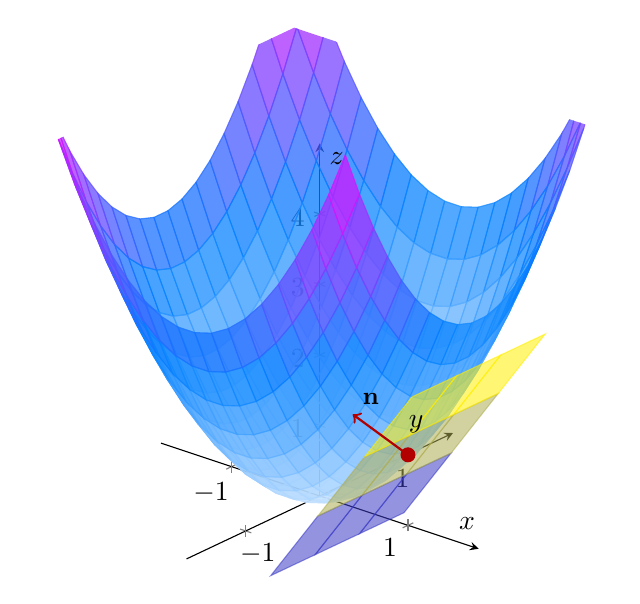
\begin{tikzpicture}
\begin{axis}[
    view={40}{25},
    xlabel={$x$}, ylabel={$y$}, zlabel={$z$},
    axis lines=center,
    tick style={thin},
    zmin=0, zmax=5,
    xtick={-2,-1,1,2}, ytick={-2,-1,1,2}, ztick={1,2,3,4},
    width=9cm, height=9cm,
]
    % Paraboloide z = x² + y²
    \addplot3[
        surf, shader=flat corner,
        samples=20, domain=-1.8:1.8,
        opacity=0.75, colormap/cool,
    ] {x^2 + y^2};
    % Punto de tangencia (1, 0, 1)
    \addplot3[only marks, mark=*, mark size=2.5pt, red!70!black]
        coordinates {(1,0,1)};
    % Plano tangente z - 1 = 2(x-1) + 0*(y-0)  →  z = 2x - 1
    % Sobre el dominio local [0.2,1.8]×[-0.9,0.9]
    \addplot3[
        surf, shader=flat,
        samples=4, domain=0.2:1.8, y domain=-0.9:0.9,
        opacity=0.55, colormap/hot,
    ] {2*x - 1};
    % Vector normal ∇F = (−2x,−2y,1) en (1,0,1) → (−2,0,1)/√5, ×0.7
    \draw[->, thick, red!70!black]
        (axis cs:1,0,1) -- (axis cs:0.374,0,1.313);
    \node[above right] at (axis cs:0.374,0,1.313)
        {\small $\mathbf{n}$};
\end{axis}
\end{tikzpicture}
\caption{Plano tangente (naranja) a $z=x^2+y^2$ en $(1,0,1)$
         con vector normal $\mathbf{n}$ perpendicular al plano}
\label{fig:plano_tangente_3d}
\end{figure}

\begin{pasos}[Protocolo para hallar el plano tangente a una superficie] Sea $z=f(x,y)$ una superficie y $P=(x_0, y_0, f(x_0, y_0))$ un punto sobre ella, estos pasos permiten calcular el plano tangente a $z$ en $P.$
\begin{enumerate}
    \item \textbf{Calcular las derivadas parciales}: Evaluar las derivadas parciales de primer orden en el punto $(x_0, y_0)$: $f_x(x_0, y_0)$ y $f_y(x_0, y_0)$.
    \item \textbf{Construir la ecuación}: Sustituir estos valores en la fórmula del plano tangente:
    \[
    z - z_0 = f_x(x_0, y_0)(x - x_0) + f_y(x_0, y_0)(y - y_0).
    \]
    \item \textbf{Simplificar (opcional)}: Reordenar la ecuación para obtener una forma más compacta, como $z = L(x, y)$.
\end{enumerate}
\end{pasos}

\begin{example}[Plano tangente al paraboloide elíptico]
Calcule el plano tangente al paraboloide elíptico $z = 2x^2 + y^2$ en el punto $(1, 1, 3)$.
\begin{myproof}
Definimos $f(x, y) = 2x^2 + y^2$. Seguimos el protocolo para hallar el plano tangente.

\begin{enumerate}
    \item \textbf{Calcular las derivadas parciales}:
    \[
    f_x(x, y) = 4x, \quad f_y(x, y) = 2y.
    \]
    Evaluando en el punto $(1, 1)$:
    \[
    f_x(1, 1) = 4, \quad f_y(1, 1) = 2.
    \]

    \item \textbf{Construir la ecuación}:
    \[
    z - 3 = 4(x - 1) + 2(y - 1).
    \]

    \item \textbf{Simplificar}:
    \[
    z = 4x + 2y - 3.
    \]

    \item \textbf{Resultado}:
    \[
    \boxed{z = 4x + 2y - 3}
    \]
\end{enumerate}
\end{myproof}
\end{example}

\begin{prob}
Calcule el plano tangente a la superficie $z = x^2 y^3$ en el punto $(1, 2)$.
\begin{myproof}
Sea $f(x,y)=x^2y^3$.

\textbf{Paso 1. Derivadas parciales.}
\[
f_x(x,y)=2xy^3,\qquad f_y(x,y)=3x^2y^2.
\]
Evaluando en $(1,2)$:
\[
f_x(1,2)=2(1)(8)=16,\quad f_y(1,2)=3(1)(4)=12,\quad f(1,2)=1\cdot 8=8.
\]

\textbf{Paso 2. Ecuación del plano tangente.}
\[
z-8=16(x-1)+12(y-2).
\]

\textbf{Paso 3. Simplificar.}
\[
z = 16x + 12y - 20.
\]

\textbf{Paso 4. Resultado.}
\[
\boxed{z=16x+12y-20}
\]
\end{myproof}
\end{prob}

\begin{rem}
El plano tangente contiene las rectas tangentes a las curvas de intersección de la superficie con los planos verticales $x = x_0$ e $y = y_0$. Específicamente, $f_x(x_0, y_0)$ y $f_y(x_0, y_0)$ son las pendientes de estas rectas tangentes en las direcciones de los ejes $x$ e $y$, respectivamente.
\end{rem}

\begin{prob}
Demuestre que el elipsoide $3x^2+2y^2+z^2=9$ y la esfera $x^2+y^2+z^2-8x-6y-8z+24=0$ son tangentes entre sí en el punto $(1,1,2)$. (Esto quiere decir que tienen un plano tangente común en ese punto.)
\begin{myproof}
\textbf{Paso 1. Plano tangente al elipsoide en $(1,1,2)$.}
Sea $F(x,y,z)=3x^2+2y^2+z^2-9$. El gradiente $\nabla F=6x\,\mathbf{i}+4y\,\mathbf{j}+2z\,\mathbf{k}$ es normal a la superficie, así que el plano tangente en $(1,1,2)$ es:
$0=6(x-1)+4(y-1)+4(z-2).$

\textbf{Paso 2. Plano tangente a la esfera en $(1,1,2)$.}
Sea $G(x,y,z)=x^2+y^2+z^2-8x-6y-8z+24$. El gradiente $\nabla G=(2x-8)\,\mathbf{i}+(2y-6)\,\mathbf{j}+(2z-8)\,\mathbf{k}$ evaluado en $(1,1,2)$: $(-6,-4,-4)$. El plano tangente es:
$0=-6(x-1)-4(y-1)-4(z-2).$

\textbf{Paso 3. Comparación de vectores normales.}
El normal al elipsoide es $\langle 6,4,4\rangle$ y el normal a la esfera es $\langle -6,-4,-4\rangle=-\langle 6,4,4\rangle$. Son paralelos (antiparalelos), luego los planos tangentes son iguales.

\textbf{Paso 4. Resultado.}
\[
\boxed{\text{Las superficies son tangentes en }(1,1,2)\text{: comparten el mismo plano tangente.}}
\]
\end{myproof}
\end{prob}

% [Original: líneas 715-723 | solución completa | sin figura]
\begin{prob}
Determine el punto del paraboloide $y=x^2+z^2$ donde el plano tangente es paralelo al plano $x+2y+3z=1.$
\begin{myproof}
\textbf{Paso 1. Gradiente de la superficie.}
Sea $F(x,y,z)=x^2+z^2-y$. Entonces $\nabla F=\langle 2x,-1,2z\rangle$ es normal al plano tangente.

\textbf{Paso 2. Condición de paralelismo.}
Para que el plano tangente sea paralelo a $x+2y+3z=1$, los normales deben ser paralelos:
$\langle 2x,-1,2z\rangle=k\langle 1,2,3\rangle.$
Despejando: $2x=k$, $-1=2k$ y $2z=3k$, luego $k=-\tfrac{1}{2}$.

\textbf{Paso 3. Coordenadas del punto.}
Con $k=-\tfrac{1}{2}$: $x_0=-\tfrac{1}{4}$, $z_0=-\tfrac{3}{4}$; sustituyendo en el paraboloide:
\[
y_0=\left(-\tfrac{1}{4}\right)^2+\left(-\tfrac{3}{4}\right)^2=\tfrac{1}{16}+\tfrac{9}{16}=\tfrac{5}{8}.
\]

\textbf{Paso 4. Resultado.}
\[
\boxed{\left(-\frac{1}{4},\,\frac{5}{8},\,-\frac{3}{4}\right)}
\]
\end{myproof}
\end{prob}

% [Original: líneas 876-882 | solución completa | sin figura]
\begin{prob}
Halle los puntos del hiperboloide $x^2-y^2-z^2=1$ donde el plano tangente es paralelo al plano $z = x + y.$
\begin{myproof}
\textbf{Paso 1. Gradiente del hiperboloide.}
Sea $F(x,y,z)=x^2-y^2-z^2-1$. El gradiente $\nabla F=\langle 2x,-2y,-2z\rangle$ es normal al plano tangente.

\textbf{Paso 2. Condición de paralelismo.}
El plano $z=x+y$ se escribe $x+y-z=0$, con normal $\langle 1,1,-1\rangle$. La condición es $\langle 2x_0,-2y_0,-2z_0\rangle=k\langle 1,1,-1\rangle$, equivalente a $\langle x_0,-y_0,-z_0\rangle=k\langle 1,1,-1\rangle$.
Luego $x_0=k$, $y_0=-k$, $z_0=k$.

\textbf{Paso 3. Sustitución en el hiperboloide.}
\[
k^2-(-k)^2-k^2=k^2-k^2-k^2=-k^2=1\implies k^2=-1.
\]
Esto es imposible en $\mathbb{R}$.

\textbf{Paso 4. Resultado.}
\[
\boxed{\text{No existe ningún punto del hiperboloide con plano tangente paralelo a }z=x+y.}
\]
\end{myproof}
\end{prob}

\section{Aproximación lineal y linealización}

Así como la recta tangente se usa para aproximar la función de una variable cerca del punto de tangencia, el plano tangente se usa para aproximar la función de dos variables cerca del punto de tangencia.

\begin{definition}[Linealización]
La \textbf{linealización} de una función $z = f(x, y)$ en un punto $(x_0, y_0)$ donde $f$ es diferenciable es la función lineal
\[
L(x, y) = f(x_0, y_0) + f_x(x_0, y_0)(x - x_0) + f_y(x_0, y_0)(y - y_0).
\]
La \textbf{aproximación lineal} correspondiente es
\[
f(x, y) \approx L(x, y),
\]
la cual es válida para puntos $(x, y)$ cercanos a $(x_0, y_0)$.
\end{definition}

\begin{example}[Linealización de $\sqrt{x^2+y^2}$]
Encuentre la linealización de la función $f(x, y) = \sqrt{x^2 + y^2}$ en el punto $(3, 4)$ y úsela para aproximar $f(3.1, 3.9)$.
\begin{myproof}
Seguimos el protocolo para hallar el plano tangente, que es equivalente a hallar la linealización.
\begin{enumerate}
    \item \textbf{Calcular las derivadas parciales}:
    \[
    f_x(x, y) = \frac{x}{\sqrt{x^2 + y^2}}, \quad f_y(x, y) = \frac{y}{\sqrt{x^2 + y^2}}.
    \]
    Evaluando en $(3, 4)$:
    \[
    f_x(3, 4) = \frac{3}{5}, \quad f_y(3, 4) = \frac{4}{5}, \quad f(3, 4) = \sqrt{9+16} = 5.
    \]

    \item \textbf{Construir la linealización}:
    \[
    L(x, y) = 5 + \frac{3}{5}(x - 3) + \frac{4}{5}(y - 4).
    \]

    \item \textbf{Simplificar}:
    \[
    L(x, y) = \frac{3x + 4y}{5}.
    \]
    \item \textbf{Aproximar y concluir}:
    \[
    f(3.1, 3.9) \approx L(3.1, 3.9) = \frac{3(3.1) + 4(3.9)}{5} = \frac{9.3 + 15.6}{5} = \frac{24.9}{5} = 4.98.
    \]
    Valor real: $\sqrt{3.1^2 + 3.9^2} \approx \sqrt{24.82} \approx 4.98197$. La linealización da $\boxed{4.98}$.
\end{enumerate}
\end{myproof}
\end{example}

\begin{prob}
Encuentre la linealización de la función $f(x, y) = \ln(1 + x + 2y)$ en el punto $(0, 0)$ y úsela para aproximar $f(0.1, -0.02)$.
\begin{myproof}
\textbf{Paso 1. Valor y derivadas en $(0,0)$.}
\[
f(0,0)=\ln 1=0.
\]
\[
f_x(x,y)=\frac{1}{1+x+2y}\implies f_x(0,0)=1;\qquad
f_y(x,y)=\frac{2}{1+x+2y}\implies f_y(0,0)=2.
\]

\textbf{Paso 2. Linealización.}
\[
L(x,y)=0+1\cdot x+2\cdot y=x+2y.
\]

\textbf{Paso 3. Aproximación.}
\[
f(0.1,-0.02)\approx L(0.1,-0.02)=0.1+2(-0.02)=0.06.
\]
Valor real: $\ln(1.06)\approx 0.0583$.

\textbf{Paso 4. Resultado.}
\[
\boxed{L(x,y)=x+2y,\quad f(0.1,-0.02)\approx 0.06}
\]
\end{myproof}
\end{prob}

\section{Diferenciales}

\begin{definition}[Diferencial total]
Para una función de dos variables $z = f(x, y)$, los diferenciales $dx$ y $dy$ son variables independientes. El \textbf{diferencial total} $dz$ (o $df$) se define como
\[
dz = f_x(x, y)\,dx + f_y(x, y)\,dy = \frac{\partial z}{\partial x}\,dx + \frac{\partial z}{\partial y}\,dy.
\]
Este diferencial representa el cambio en la \emph{linealización} $L(x,y)$ cuando las variables independientes cambian en $dx$ y $dy$. Si $dx = \Delta x$ y $dy = \Delta y$ son pequeños, entonces $\Delta z \approx dz$.
\end{definition}

\begin{figure}[H]
\centering
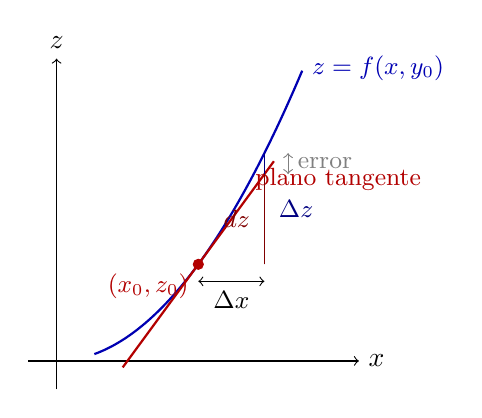
\begin{tikzpicture}[scale=1.2]
    \draw[thin,->] (-0.3,0) -- (3.2,0) node[right] {$x$};
    \draw[thin,->] (0,-0.3) -- (0,3.2) node[above] {$z$};
    % Curva z = x² (sección de la superficie en y=y0)
    \draw[thick, blue!70!black, domain=0.4:2.6, samples=50, smooth, variable=\t]
        plot ({\t}, {\t*\t/2.2});
    \node[anchor=west, blue!70!black] at (2.6,3.1) {\small $z=f(x,y_0)$};
    % Punto (x0, z0)
    \pgfmathsetmacro{\xo}{1.5}
    \pgfmathsetmacro{\zo}{1.5*1.5/2.2}
    \filldraw[red!70!black] (\xo,\zo) circle (1.5pt)
        node[anchor=north east] {\small $(x_0,z_0)$};
    % Plano tangente (recta tangente en 2D)
    % Pendiente: (d/dx)(x²/2.2) = 2x/2.2 = x/1.1; en x=1.5: m=1.5/1.1≈1.364
    \pgfmathsetmacro{\m}{1.5/1.1}
    \draw[thick, red!70!black]
        ({1.5-0.8},{\zo - \m*0.8}) -- ({1.5+0.8},{\zo + \m*0.8});
    \node[anchor=south west, red!70!black] at ({1.5+0.5},{\zo+\m*0.5})
        {\small plano tangente};
    % Δx
    \pgfmathsetmacro{\dx}{0.7}
    \draw[thin, <->] (\xo, \zo-0.18) -- (\xo+\dx, \zo-0.18)
        node[midway, below] {\small $\Delta x$};
    % Δz (cambio real en la curva)
    \pgfmathsetmacro{\znew}{(\xo+\dx)*(\xo+\dx)/2.2}
    \draw[thin, blue!50!black]
        (\xo+\dx, \zo) -- (\xo+\dx, \znew);
    \node[anchor=west, blue!50!black] at (\xo+\dx+0.05, {(\zo+\znew)/2})
        {\small $\Delta z$};
    % dz (cambio en el plano tangente)
    \pgfmathsetmacro{\dz}{\m*\dx}
    \draw[thin, red!50!black]
        (\xo+\dx, \zo) -- (\xo+\dx, \zo+\dz);
    \node[anchor=east, red!50!black] at (\xo+\dx-0.05, {\zo+\dz/2})
        {\small $dz$};
    % Separación entre dz y Δz (error)
    \draw[thin, gray, <->] (\xo+\dx+0.25, \zo+\dz) -- (\xo+\dx+0.25, \znew)
        node[midway, right] {\small error};
\end{tikzpicture}
\caption{Aproximación lineal: $dz$ (plano tangente) aproxima $\Delta z$
         (cambio real en la superficie) para incrementos pequeños $\Delta x$}
\label{fig:aprox_lineal_dz}
\end{figure}

\begin{rem}
La definición de diferencial se extiende de manera natural a funciones de más variables. Por ejemplo, para $w = f(x, y, z)$,
\[
dw = f_x \, dx + f_y \, dy + f_z \, dz.
\]
\end{rem}

\begin{rem}
La noción de diferenciabilidad formaliza la condición bajo la cual un plano tangente existe y la aproximación lineal es buena. Una función es diferenciable en un punto si su incremento $\Delta z$ puede escribirse como la combinación lineal dada por el diferencial total más un error que tiende a cero más rápido que la distancia al punto.
\end{rem}

\begin{theorem}[Diferenciabilidad y continuidad]
Si $f$ es diferenciable en un punto $(x_0, y_0)$, entonces $f$ es continua en ese punto.
\end{theorem}
\begin{proof}
\textbf{Paso 1. Escribir el incremento.} Por definición de diferenciabilidad en
$(x_0,y_0)$, el incremento $\Delta z=f(x_0+\Delta x,\,y_0+\Delta y)-f(x_0,y_0)$
puede escribirse como
\[
  \Delta z=f_x(x_0,y_0)\,\Delta x+f_y(x_0,y_0)\,\Delta y
           +\varepsilon_1\,\Delta x+\varepsilon_2\,\Delta y,
\]
donde $\varepsilon_1,\varepsilon_2\to 0$ cuando $(\Delta x,\Delta y)\to(0,0)$.

\textbf{Paso 2. Tomar el límite.} Cada uno de los cuatro sumandos es el producto
de un factor acotado (las parciales, constantes en el punto fijo, o los
$\varepsilon_i\to 0$) por $\Delta x$ o $\Delta y$, factores que tienden a $0$.
En consecuencia
\[
  \lim_{(\Delta x,\Delta y)\to(0,0)}\Delta z=0.
\]

\textbf{Paso 3. Concluir.} Esto equivale a
$\displaystyle\lim_{(\Delta x,\Delta y)\to(0,0)}f(x_0+\Delta x,\,y_0+\Delta y)=f(x_0,y_0)$,
que es precisamente la continuidad de $f$ en $(x_0,y_0)$.
\end{proof}

\begin{theorem}[Criterio de diferenciabilidad]
Si las derivadas parciales $f_x$ y $f_y$ existen en una región que contiene a $(x_0, y_0)$ y son continuas en $(x_0, y_0)$, entonces $f$ es diferenciable en $(x_0, y_0)$.
\end{theorem}

\begin{example}[Diferenciabilidad de $xe^{xy}$]
Demuestre que la función $f(x, y) = x e^{xy}$ es diferenciable en $(1, 0)$ y determine su linealización. Luego úsela para aproximar $f(1.1, -0.1)$.
\begin{myproof}
\begin{enumerate}
    \item \textbf{Calcular las derivadas parciales}:
    \[
    f_x(x, y) = e^{xy} + xy e^{xy}, \quad f_y(x, y) = x^2 e^{xy}.
    \]
    Estas funciones son continuas en todo $\mathbb{R}^2$ por ser combinaciones de funciones continuas ($e^{xy}$ es continua por ser composición de la exponencial con un polinomio). Por lo tanto, $f$ es diferenciable en $(1, 0)$.
    Evaluando en $(1, 0)$:
    \[
    f(1, 0) = 1,\quad f_x(1, 0) = 1,\quad f_y(1, 0) = 1.
    \]

    \item \textbf{Construir la linealización}:
    \[
    L(x, y) = 1 + 1(x - 1) + 1(y - 0) = x + y.
    \]

    \item \textbf{Aproximar}:
    \[
    f(1.1, -0.1) \approx L(1.1, -0.1) = 1.0.
    \]

    \item \textbf{Resultado.}
    \[
    \boxed{L(x, y) = x + y,\quad f(1.1, -0.1) \approx 1.0}
    \]
\end{enumerate}
\end{myproof}
\end{example}


\section{Problemas propuestos}

% Básico
\begin{prob}
Calcule las primeras derivadas parciales de las siguientes funciones:
\begin{multicols}{2}
\begin{enumerate}
    \item $f(x,y)=x^3-3x^2 y+2y^3$
    \item $f(x,y)=e^{x^2+y^2}$
    \item $f(x,y)=\ln(x^2+y^2+1)$
    \item $f(x,y)=\arctan(y/x)$
    \item $f(x,y)=\sin(x^2 y)$
    \item $f(x,y)=x^y$ ($x>0$)
    \item $f(x,y,z)=x^2 y z^3$
    \item $f(x,y,z)=\ln(x^2+y^2+z^2)$
\end{enumerate}
\end{multicols}
\end{prob}

\begin{prob}
Sea $f(x,y)=\displaystyle\int_x^y \sqrt{1+t^3}\,dt$. Calcule $f_x$ y $f_y$
aplicando el Teorema Fundamental del Cálculo (observe que $x$ es el límite
inferior y $y$ el superior).
\end{prob}

\begin{prob}
Calcule todas las derivadas parciales de segundo orden de:
\begin{multicols}{2}
\begin{enumerate}
    \item $f(x,y)=x^3 y^2$
    \item $f(x,y)=e^x\cos y$
    \item $f(x,y)=\ln(x^2+y^2)$
    \item $f(x,y)=\sin(x+y)$
\end{enumerate}
\end{multicols}
\end{prob}

\begin{prob}
Verifique el Teorema de Clairaut para $f(x,y)=x^2 e^{xy}$ calculando
$f_{xy}$ y $f_{yx}$.
\end{prob}


% Intermedio
\begin{prob}
Determine si cada afirmación es verdadera o falsa. Justifique.
\begin{enumerate}
    \item Si $f$ es continua en $(a,b)$, entonces $f_x$ y $f_y$ existen
    en $(a,b)$.
    \item Si $f_x$ y $f_y$ existen en $(a,b)$, entonces $f$ es continua
    en $(a,b)$.
    \item Si $f_{xy}=f_{yx}$ en todo punto, entonces $f$ es continua.
\end{enumerate}
\end{prob}

\begin{prob}
Encuentre la ecuación del plano tangente a la superficie $xy+yz+zx=7$ en el punto $(-1,3,5).$
\end{prob}


\begin{prob}
Encuentre la ecuación del plano tangente a la superficie $x^2+2y^2+4z^2=9$ en el punto $(2,1,\sqrt{3}/2).$
\end{prob}

\begin{prob}
Encuentre la ecuación del plano tangente a la superficie $5x^2-y^2+4z^2=8$ en el punto $(-2,4,1).$
\end{prob}

\begin{prob}
Considere la función $f(x,y)=3x^2y^4-12x^6+2xy^5.$ Calcule $\dfrac{\partial f}{\partial x}$ y $\dfrac{\partial f}{\partial y}$ para verificar que \[  x\left( \dfrac{\partial f}{\partial x} \right)+y\left( \dfrac{\partial f}{\partial y} \right)=6f(x,y).\] 
\end{prob}

\begin{prob}
Una función de dos variables $f(x,y)$ que satisface la ecuación de Laplace, \[\dfrac{\partial^2f}{\partial x^2}+\dfrac{\partial^2f}{\partial y^2}=0\] se dice que es armónica. Determine si la función $f(x,y)=Ay^3+5x$ es armónica.
\end{prob}

\begin{prob}
Encuentre la ecuación del plano tangente a la superficie $x^2+2y^2+z^2=4$ en el punto $(1,-1,1).$
\end{prob}

\begin{prob}
Si la ecuación $F(x,y,z)=x^3+y^3+z^3-3xyz=0$ define implícitamente $z=z(x,y)$, encuentre
$\dfrac{\partial z}{\partial x}$ y $\dfrac{\partial z}{\partial y}$ en el punto $(1,1,1)$.
\end{prob}

\begin{prob}
El volumen de una caja rectangular es $V=xyz$. Interprete $\partial V/\partial y$
como la razón de cambio del volumen respecto al ancho $y$ manteniendo $x$ y $z$
fijos; calcúlela, evalúela en $(x,y,z)=(3,4,2)$ e indique sus unidades cuando
las longitudes se miden en centímetros.
\end{prob}

\begin{prob}
Halle la linealización $L(x,y,z)$ de $f(x,y,z)=x^3yz$ en el punto $(1,2,1)$ y
úsela para aproximar $f(1{,}05,\;1{,}9,\;1{,}1)$.
\end{prob}


% Desafiante
\begin{prob}
Los lados de un rectángulo se miden como $x=4{,}00\;\text{cm}$ y $y=3{,}00\;\text{cm}$
con posibles errores $|\Delta x|\le 0{,}05\;\text{cm}$ y $|\Delta y|\le 0{,}03\;\text{cm}$.
Use diferenciales para estimar el error máximo en el área $A=xy$.
\end{prob}

\begin{prob}
Encuentre el plano tangente a la superficie implícita $x^2 y+y^2 z+z^2 x=3$ en el
punto $(1,1,1)$.
\end{prob}

\begin{prob}
Sea $w=x^2 e^{y/z}$. Calcule el diferencial total $dw$ y úselo para estimar el cambio
en $w$ cuando $(x,y,z)$ pasa de $(2,\,0,\,1)$ a $(2{,}1,\;0{,}1,\;0{,}9)$.
\end{prob}

\begin{prob}
Si $z$ está definida implícitamente por la ecuación $e^z-z=xy+1$,
encuentre $\dfrac{\partial z}{\partial x}$ y $\dfrac{\partial z}{\partial y}$.
\end{prob}

\begin{prob}
Sea $z=f(x,y)$ diferenciable. Sobre la superficie considere las curvas
coordenadas $\mathbf r_1(x)=(x,y_0,f(x,y_0))$ y $\mathbf r_2(y)=(x_0,y,f(x_0,y))$.
Muestre que sus vectores tangentes en $(x_0,y_0)$ son
$\mathbf T_x=\langle 1,0,f_x\rangle$ y $\mathbf T_y=\langle 0,1,f_y\rangle$, y que
$\mathbf T_x\times\mathbf T_y=\langle -f_x,-f_y,1\rangle$ es el vector normal del
plano tangente.
\end{prob}

\begin{prob}
Deduzca que el plano tangente al elipsoide
$\dfrac{x^2}{a^2}+\dfrac{y^2}{b^2}+\dfrac{z^2}{c^2}=1$ en un punto
$(x_0,y_0,z_0)$ de la superficie es
$\dfrac{x x_0}{a^2}+\dfrac{y y_0}{b^2}+\dfrac{z z_0}{c^2}=1$.
(Sugerencia: use $\nabla F$ y que el punto satisface la ecuación del elipsoide.)
\end{prob}

% ============================================================
